\begin{frame}{Diagonal Flip}
    \begin{figure}[scale=0.5]
        \centering
        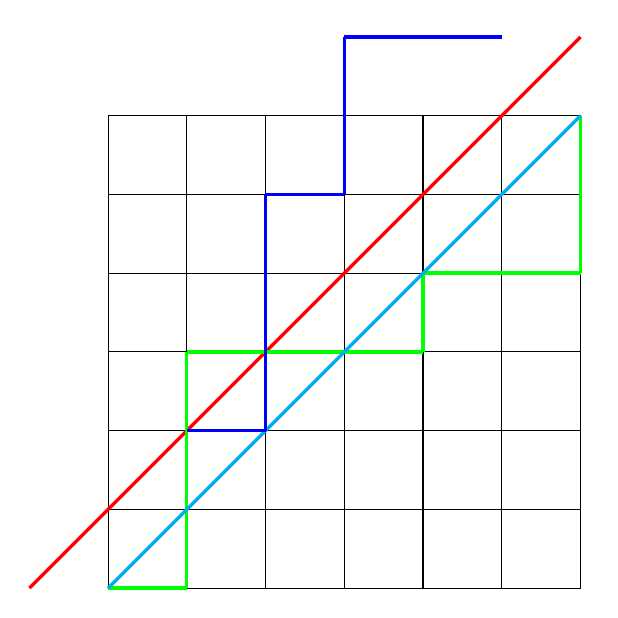
\begin{tikzpicture}
            \draw (0, 0)--(6, 0);
            \draw (6, 0)--(6, 6);
            \draw (6, 6)--(0, 6);
            \draw (0, 6)--(0, 0);
            \draw (0, 0)--(6, 0);
            \draw (0, 1)--(6, 1);
            \draw (0, 2)--(6, 2);
            \draw (0, 3)--(6, 3);
            \draw (0, 4)--(6, 4);
            \draw (0, 5)--(6, 5);
            \draw (0, 0)--(0, 6);
            \draw (1, 0)--(1, 6);
            \draw (2, 0)--(2, 6);
            \draw (3, 0)--(3, 6);
            \draw (4, 0)--(4, 6);
            \draw (5, 0)--(5, 6);
            \draw (-1, 0)--(6, 7) [red, very thick];
            \draw (0, 0)--(1, 0)[green, very thick];
            \draw (1, 0)--(1, 3)[green, very thick];
            \draw (4, 3)--(1, 3)[green, very thick];
            \draw (4, 3)--(4, 4)[green, very thick];
            \draw (6, 4)--(4, 4)[green, very thick];
            \draw (6, 6)--(6, 4)[green, very thick];
            \draw (6, 6)--(0, 0)[cyan, very thick];
            \draw (1, 2)--(2, 2)[blue, very thick];
            \draw (2, 2)--(2, 5)[blue, very thick];
            \draw (2, 5)--(3, 5)[blue, very thick];
            \draw (3, 5)--(3, 7)[blue, very thick];
            \draw (3, 7)--(5, 7)[blue, very thick];
            \draw (1, 2)node(1)[minimum size = 2mm, blue]{};
            \draw (5, 7)node(2)[minimum size = 2mm, blue]{};
            \draw (6, 6)node(3)[minimum size = 2mm, green]{};
        \end{tikzpicture}
    \end{figure}
\end{frame}

\begin{frame}{Diagonal Flip}
    \begin{itemize}[<+->]
        \item In the figure any path crossing the light blue diagonal is a {\bf{bad path}} i.e., they cross the diagonal.
        \item Observe that any bad path first touches the red line
        \item Now whenever a path touches the red line for the first time let us flip that path after that point about the red line. So all the bad paths get flipped and none of the good paths get flipped.
        \item What is the final point where all the flipped paths reach?
        \item They will reach to the point (n-1, n+1).
        \item So number of bad paths = paths from (0, 0) to (n-1, n+1) = ${2n \choose n-1}$
        \item Hence Proved!!
    \end{itemize}
\end{frame}